\chapter{Knapsack Problem 0/1}
Questione da risolvere: trovare il subset di oggetti di massimo valore complessivo
che non superi la capacità C.
\paragraph*{Oggetti} Ad ogni oggetto viene associato un peso e un valore, quindi il problema
consiste nel inserire nello zaino il massimo valore possibile senza superare il peso massimo.
\begin{center}
    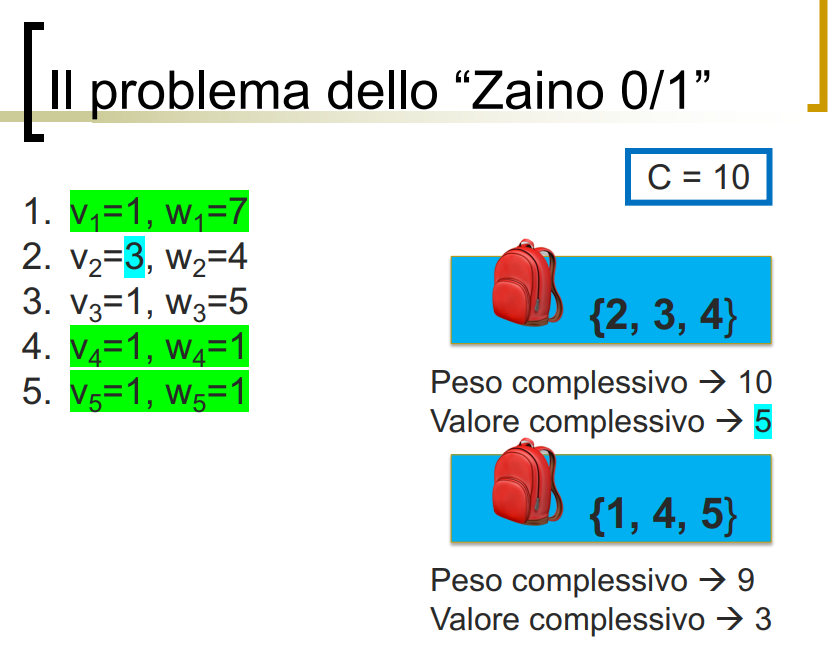
\includegraphics[width=100mm, scale=0.5]{chapters_ulerich/img/knapsack_example.png}
\end{center}

